% *** Authors should verify (and, if needed, correct) their LaTeX system  ***
% *** with the testflow diagnostic prior to trusting their LaTeX platform ***
% *** with production work. IEEE's font choices can trigger bugs that do  ***
% *** not appear when using other class files.                            ***
% The testflow support page is at:
% http://www.michaelshell.org/tex/testflow/


%%*************************************************************************
%% Legal Notice:
%% This code is offered as-is without any warranty either expressed or
%% implied; without even the implied warranty of MERCHANTABILITY or
%% FITNESS FOR A PARTICULAR PURPOSE!
%% User assumes all risk.
%% In no event shall IEEE or any contributor to this code be liable for
%% any damages or losses, including, but not limited to, incidental,
%% consequential, or any other damages, resulting from the use or misuse
%% of any information contained here.
%%
%% All comments are the opinions of their respective authors and are not
%% necessarily endorsed by the IEEE.
%%
%% This work is distributed under the LaTeX Project Public License (LPPL)
%% ( http://www.latex-project.org/ ) version 1.3, and may be freely used,
%% distributed and modified. A copy of the LPPL, version 1.3, is included
%% in the base LaTeX documentation of all distributions of LaTeX released
%% 2003/12/01 or later.
%% Retain all contribution notices and credits.
%% ** Modified files should be clearly indicated as such, including  **
%% ** renaming them and changing author support contact information. **
%%
%% File list of work: IEEEtran.cls, New_IEEEtran_how-to.pdf, bare_jrnl_new_sample4.tex,
%%*************************************************************************
\PassOptionsToPackage{unicode}{hyperref}
\PassOptionsToPackage{hyphens}{url}
\PassOptionsToPackage{dvipsnames,svgnames,x11names}{xcolor}
% Note that the a4paper option is mainly intended so that authors in
% countries using A4 can easily print to A4 and see how their papers will
% look in print - the typesetting of the document will not typically be
% affected with changes in paper size (but the bottom and side margins will).
% Use the testflow package mentioned above to verify correct handling of
% both paper sizes by the user's LaTeX system.
%
% Also note that the "draftcls" or "draftclsnofoot", not "draft", option
% should be used if it is desired that the figures are to be displayed in
% draft mode.
%
\documentclass[
  journal,
]{IEEEtran}%
% If IEEEtran.cls has not been installed into the LaTeX system files,
% manually specify the path to it like:
% \documentclass[journal]{../sty/IEEEtran}
\usepackage[cmex10]{amsmath}
\usepackage{amssymb}
\usepackage{iftex}
\ifPDFTeX
  \usepackage[T1]{fontenc}
  \usepackage[utf8]{inputenc}
  \usepackage{textcomp} % provide euro and other symbols
\else % if luatex or xetex
  \usepackage{unicode-math} % this also loads fontspec
  \defaultfontfeatures{Scale=MatchLowercase}
  \defaultfontfeatures[\rmfamily]{Ligatures=TeX,Scale=1}
\fi
%\usepackage{lmodern}
\ifPDFTeX\else
\fi
% Use upquote if available, for straight quotes in verbatim environments
\IfFileExists{upquote.sty}{\usepackage{upquote}}{}
\IfFileExists{microtype.sty}{% use microtype if available
  \usepackage[]{microtype}
  \UseMicrotypeSet[protrusion]{basicmath} % disable protrusion for tt fonts
}{}
\makeatletter
\parindent    1.0em
\ifCLASSOPTIONcompsoc
  \parindent    1.5em
\fi
\makeatother
\usepackage{xcolor}
\setlength{\emergencystretch}{3em} % prevent overfull lines

\setcounter{secnumdepth}{5}
% Make \paragraph and \subparagraph free-standing
\ifx\paragraph\undefined\else
  \let\oldparagraph\paragraph
  \renewcommand{\paragraph}[1]{\oldparagraph{#1}\mbox{}}
\fi
\ifx\subparagraph\undefined\else
  \let\oldsubparagraph\subparagraph
  \renewcommand{\subparagraph}[1]{\oldsubparagraph{#1}\mbox{}}
\fi


\providecommand{\tightlist}{%
  \setlength{\itemsep}{0pt}\setlength{\parskip}{0pt}}\usepackage{longtable,booktabs,array}
\usepackage{calc} % for calculating minipage widths
% Correct order of tables after \paragraph or \subparagraph
\usepackage{etoolbox}
\makeatletter
\patchcmd\longtable{\par}{\if@noskipsec\mbox{}\fi\par}{}{}
\makeatother
% Allow footnotes in longtable head/foot
\IfFileExists{footnotehyper.sty}{\usepackage{footnotehyper}}{\usepackage{footnote}}
\makesavenoteenv{longtable}
\usepackage{graphicx}
\makeatletter
\def\maxwidth{\ifdim\Gin@nat@width>\linewidth\linewidth\else\Gin@nat@width\fi}
\def\maxheight{\ifdim\Gin@nat@height>\textheight\textheight\else\Gin@nat@height\fi}
\makeatother
% Scale images if necessary, so that they will not overflow the page
% margins by default, and it is still possible to overwrite the defaults
% using explicit options in \includegraphics[width, height, ...]{}
\setkeys{Gin}{width=\maxwidth,height=\maxheight,keepaspectratio}
% Set default figure placement to htbp
\makeatletter
\def\fps@figure{htbp}
\makeatother
\newlength{\cslhangindent}
\setlength{\cslhangindent}{1.5em}
\newlength{\csllabelwidth}
\setlength{\csllabelwidth}{3em}
\newlength{\cslentryspacingunit} % times entry-spacing
\setlength{\cslentryspacingunit}{\parskip}
\newenvironment{CSLReferences}[2] % #1 hanging-ident, #2 entry spacing
 {% don't indent paragraphs
  \setlength{\parindent}{0pt}
  % turn on hanging indent if param 1 is 1
  \ifodd #1
  \let\oldpar\par
  \def\par{\hangindent=\cslhangindent\oldpar}
  \fi
  % set entry spacing
  \setlength{\parskip}{#2\cslentryspacingunit}
 }%
 {}
\usepackage{calc}
\newcommand{\CSLBlock}[1]{#1\hfill\break}
\newcommand{\CSLLeftMargin}[1]{\parbox[t]{\csllabelwidth}{#1}}
\newcommand{\CSLRightInline}[1]{\parbox[t]{\linewidth - \csllabelwidth}{#1}\break}
\newcommand{\CSLIndent}[1]{\hspace{\cslhangindent}#1}

\usepackage{physics}
\usepackage[version=3]{mhchem}
\usepackage{orcidlink}
\usepackage{float}
\floatplacement{table}{htb}
\makeatletter
\makeatother
\makeatletter
\makeatother
\makeatletter
\@ifpackageloaded{caption}{}{\usepackage{caption}}
\AtBeginDocument{%
\ifdefined\contentsname
  \renewcommand*\contentsname{Table of contents}
\else
  \newcommand\contentsname{Table of contents}
\fi
\ifdefined\listfigurename
  \renewcommand*\listfigurename{List of Figures}
\else
  \newcommand\listfigurename{List of Figures}
\fi
\ifdefined\listtablename
  \renewcommand*\listtablename{List of Tables}
\else
  \newcommand\listtablename{List of Tables}
\fi
\ifdefined\figurename
  \renewcommand*\figurename{Fig.}
\else
  \newcommand\figurename{Fig.}
\fi
\ifdefined\tablename
  \renewcommand*\tablename{Table}
\else
  \newcommand\tablename{Table}
\fi
}
\@ifpackageloaded{float}{}{\usepackage{float}}
\floatstyle{ruled}
\@ifundefined{c@chapter}{\newfloat{codelisting}{h}{lop}}{\newfloat{codelisting}{h}{lop}[chapter]}
\floatname{codelisting}{Listing}
\newcommand*\listoflistings{\listof{codelisting}{List of Listings}}
\makeatother
\makeatletter
\@ifpackageloaded{caption}{}{\usepackage{caption}}
\@ifpackageloaded{subcaption}{}{\usepackage{subcaption}}
\makeatother
\makeatletter
\@ifpackageloaded{tcolorbox}{}{\usepackage[skins,breakable]{tcolorbox}}
\makeatother
\makeatletter
\@ifundefined{shadecolor}{\definecolor{shadecolor}{rgb}{.97, .97, .97}}
\makeatother
\makeatletter
\makeatother
\makeatletter
\makeatother
\usepackage[skip=2pt,font=footnotesize]{caption}
%\captionsetup{format=myformat}
\makeatletter
%\setlength{\cslhangindent}{0pt plus .5pt}
\providecommand{\bibfont}{\footnotesize}
\let\CSLReferences@rig=\CSLReferences
\renewcommand{\CSLReferences}[2]{
\bibfont\settowidth\csllabelwidth{[999]}
\CSLReferences@rig{#1}{#2}
\vskip 0.3\baselineskip plus 0.1\baselineskip minus 0.1\baselineskip%
}
\makeatother
\ifLuaTeX
  \usepackage{selnolig}  % disable illegal ligatures
\fi
\IfFileExists{bookmark.sty}{\usepackage{bookmark}}{\usepackage{hyperref}}
\IfFileExists{xurl.sty}{\usepackage{xurl}}{} % add URL line breaks if available
\urlstyle{same} % disable monospaced font for URLs
\hypersetup{
  pdftitle={Optimierung der Preisstrategien bei Airbnb: Eine Analyse zur Maximierung der Einnahmen},
  pdfauthor={Cedric Gisler \& Jovan Pajic},
  colorlinks=true,
  linkcolor={blue},
  filecolor={Maroon},
  citecolor={Blue},
  urlcolor={Blue},
  pdfcreator={LaTeX via pandoc}}

% *** Do not adjust lengths that control margins, column widths, etc. ***
% *** Do not use packages that alter fonts (such as pslatex).         ***
% There should be no need to do such things with IEEEtran.cls V1.6 and later.
% (Unless specifically asked to do so by the journal or conference you plan
% to submit to, of course. )


% correct bad hyphenation here
\hyphenation{op-tical net-works semi-conduc-tor}

%
% paper title
% can use linebreaks \\ within to get better formatting as desired
% Do not put math or special symbols in the title.
% paper title
% can use linebreaks \\ within to get better formatting as desired
% Do not put math or special symbols in the title.
\title{Optimierung der Preisstrategien bei Airbnb: Eine Analyse zur
Maximierung der Einnahmen}

\author{
Cedric Gisler \& Jovan Pajic%

}
\begin{document}

% The paper headers

% use for special paper notices

% make the title area
\maketitle

% As a general rule, do not put math, special symbols or citations
% in the abstract or keywords.
% Note that keywords are not normally used for peerreview papers.

% For peer review papers, you can put extra information on the cover
% page as needed:
% \ifCLASSOPTIONpeerreview
% \begin{center} \bfseries EDICS Category: 3-BBND \end{center}
% \fi
%
% For peerreview papers, this IEEEtran command inserts a page break and
% creates the second title. It will be ignored for other modes.
% \IEEEpeerreviewmaketitle

\ifdefined\Shaded\renewenvironment{Shaded}{\begin{tcolorbox}[frame hidden, interior hidden, sharp corners, breakable, enhanced, boxrule=0pt, borderline west={3pt}{0pt}{shadecolor}]}{\end{tcolorbox}}\fi

\hypertarget{abstrakt}{%
\section{1. Abstrakt}\label{abstrakt}}

Lorem ipsum dolor sit amet, consetetur sadipscing elitr, sed diam nonumy
eirmod tempor invidunt ut labore et dolore magna aliquyam erat, sed diam
voluptua. At vero eos et accusam et justo duo dolores et ea rebum. Stet
clita kasd gubergren, no sea takimata sanctus est Lorem ipsum dolor sit
amet. Lorem ipsum dolor sit amet, consetetur sadipscing elitr, sed diam
nonumy eirmod tempor invidunt ut labore et dolore magna aliquyam erat,
sed diam voluptua. At vero eos et accusam et justo duo dolores et ea
rebum. Stet clita kasd gubergren, no sea takimata sanctus est Lorem
ipsum dolor sit amet. Lorem ipsum dolor sit amet, consetetur sadipscing
elitr, sed diam nonumy eirmod tempor invidunt ut labore et dolore magna
aliquyam erat, sed diam voluptua. At vero eos et accusam et justo duo
dolores et ea rebum. Stet clita kasd gubergren, no sea takimata sanctus
est Lorem ipsum dolor sit amet.

\hypertarget{einleitung-mit-forschungsfrage-d.h.-geschuxe4ftsfrage-am-ende}{%
\section{2. Einleitung (mit Forschungsfrage (d.h. Geschäftsfrage) am
Ende)}\label{einleitung-mit-forschungsfrage-d.h.-geschuxe4ftsfrage-am-ende}}

In der heutigen, schnelllebigen Welt des Online-Tourismus spielen
Plattformen wie Airbnb eine zentrale Rolle bei der Art und Weise, wie
Menschen reisen und Unterkünfte buchen. Airbnb bietet eine Vielzahl von
Unterkünften an, von einfachen Zimmern bis hin zu luxuriösen Villen. So
vielfältig wie das Angebot sind auch die Vorlieben und Erwartungen der
Gäste. Vor diesem Hintergrund stellt sich die Forschungsfrage:
\textbf{\emph{Welche Eigenschaften einer Airbnb-Unterkunft ziehen Gäste
an und ermöglichen es, einen höheren Preis pro Apparment zu erzielen?}}

Der grösste Unterschied eines Airbnbs ist deren Grösse. Eine der
wichtigsten Eigenschaften eines Apartments ist aber die Lage, die
Bewertung und der Gastgeber, somit definieren wir folgende
Nullhypothesen:

\begin{enumerate}
\def\labelenumi{\arabic{enumi}.}
\item
  \textbf{Bewertung der Airbnb-Unterkünften:}

  \begin{itemize}
  \item
    \textbf{Nullhypothese (H0)}: Die Höhe der Bewertung hat keinen
    Einfluss auf die Höhe des Preises pro Person der Unterkunft.
  \item
    \textbf{Alternativhypothese (H1)}: Die Höhe der Bewertung hat einen
    Einfluss auf die Höhe des Preises pro Person der Unterkunft.
  \end{itemize}
\item
  \textbf{Gastgeber der Airbnb-Unterkunft:}

  \begin{itemize}
  \item
    \textbf{Nullhypothese (H0)}: Die Informationen über den Host, wie
    ``host\_is\_superhost'', ``host\_identifiy\_verified'' und
    ``host\_listings\_count'' haben keinen Einfluss auf die Höhe des
    Preises pro Person der Unterkunft.
  \item
    \textbf{Alternativhypothese (H1)}: Die Informationen über den Host,
    wie ``host\_is\_superhost'', ``host\_identifiy\_verified'' und
    ``host\_listings\_count'' haben einen Einfluss auf die Höhe des
    Preises pro Person der Unterkunft.
  \end{itemize}
\item
  \textbf{Lage des Airbnb:}

  \begin{itemize}
  \item
    \textbf{Nullhypothese (H0)}: Die Nähe zum Stadtzentrum hat keinen
    Einfluss auf die Höhe des Preises pro Person der Unterkunft.
  \item
    \textbf{Alternativhypothese (H1)}: Die Nähe zum Stadtzentrum hat
    einen Einfluss auf die Höhe des Preises pro Person der Unterkunft.
  \end{itemize}
\end{enumerate}

Weitere wichtige Eigenschaften sind Ereignisse (z.B. Zürich:
Streetparade, Zürich Film Festival) in der betreffenden Stadt. Da wir
aber die Daten nur zu einem einzelnen Zeitpunkt haben und keine
Zeitserie, können wir den Einfluss dieser Ereignisse auf den Preis pro
Person der Unterkunft nicht untersuchen.

\textbf{Deskriptive Analyse:} Wir möchten überprüfen, ob unsere
Hypothesen so stimmen und wir mit unserer Annahme über die Einflüsse auf
den Preis pro Person der Unterkunft richtig liegen.

\textbf{Prädiktive Analyse:} Wir möchten den Trend des Preises pro
Person der Unterkunft aufzeigen und untersuchen, ob wir mithilfe der
Bewertung und den wichtigsten Eigenschaften einer Unterkunft eine
Prognose über den Preis machen können.

\textbf{Präskriptive Analyse:} Wir möchten zeigen, welche Eigenschaften
wie verbessert werden müssen, um die Preise pro Person der Unterkunft
signifikant erhöhen zu können, um einen höheren Preis erzielen zu
können.

\hypertarget{datenquelle-mit-angaben-zu-quelle-qualituxe4t-und-bereinigungsschritten-der-daten}{%
\section{3. Datenquelle (mit Angaben zu Quelle, Qualität und
Bereinigungsschritten der
Daten)}\label{datenquelle-mit-angaben-zu-quelle-qualituxe4t-und-bereinigungsschritten-der-daten}}

Die Daten für diese Analyse stammen von der Inside Airbnb Organisation
\protect\hyperlink{ref-inside-airbnb-2023}{{[}1{]}}, die sich dafür
einsetzt, ihre Gemeinden vor den negativen Auswirkungen von
Kurzzeitvermietungen zu schützen. Diese Organisation sammelt und
veröffentlicht regelmässig aktualisierte Datensätze, die aus öffentlich
verfügbaren Informationen auf der Airbnb-Website stammen. Diese
Datensätze würden wir als Vertrauenswürdig einstufen.

Die extrahierten Datensätze umfassen Informationen aus drei bedeutenden
Regionen in der Schweiz: Zürich (27. Dezember 2023), Genénve (27.
Dezember 2023) und Vaud (10. März 2024).

Die Daten umfassen verschiedene Dateien für jede Stadt, wobei für die
Analyse hauptsächlich das ``listings\_long.csv''-File verwendet wird, da
es für die Geschäftsfragen relevant ist. Die Qualität der Daten in
diesem File ist insgesamt sehr hoch, mit wenigen leeren Feldern und
einer konsistenten Struktur innerhalb der Spalten.

Es werden insgesamt 3 Datensätze verwendet, die dieselbe Struktur
aufweisen, jedoch aus drei verschiedenen Regionen stammen, die wir hier
analysieren möchten.

Einige Spalten, wie ``description'', ``neighborhood\_overview'',
``host\_neighborhood'', ``neighborhood'', und die Beschreibung der
Liegenschaft, wie ``bathrooms'' und ``bedrooms'', weisen eine
beträchtliche Anzahl leerer Felder auf. Es wird vermutet, dass diese
Felder optional für die Gastgeber sind und daher nicht immer ausgefüllt
werden. Ebenso fehlt bei einigen Einträgen der Preis, was eine Analyse
erfordert, um mögliche Korrelationen mit anderen Feldern, wie dem ersten
Review, zu identifizieren.

Trotz dieser kleinen Unregelmässigkeiten ist die Datenqualität insgesamt
hoch, und die Beschreibung der Datenfelder wird durch das Data
Dictionary \protect\hyperlink{ref-inside-airbnb-2022}{{[}2{]}} gut
unterstützt.

\textbf{Datenbereinigungsschritte:}

\begin{enumerate}
\def\labelenumi{\arabic{enumi}.}
\item
  \textbf{Entfernung irrelevanter oder leerer Spalten:} Vor der Analyse
  wurden alle Spalten entfernt, die für die Fragestellungen nicht
  relevant sind oder leere Felder enthalten.
\item
  \textbf{Überprüfung der Einheitlichkeit und Konsistenz der Werte:} Die
  verbleibenden Spalten wurden auf Einheitlichkeit der Werte und
  Konsistenz der ``N/A''-Kennzeichnungen überprüft, um sicherzustellen,
  dass die Daten konsistent und interpretierbar sind.
\item
  \textbf{Analyse von Einträgen ohne Preisangabe:} Einige Einträge
  weisen keine Preisangabe auf, was eine Analyse erfordert, um mögliche
  Korrelationen mit anderen Feldern, wie dem ersten Review, zu
  identifizieren. Je nach Ergebnis dieser Analyse könnten Einträge ohne
  Preisangabe entfernt oder anderweitig behandelt werden, um die
  Datenintegrität zu gewährleisten.
\end{enumerate}

\hypertarget{datenqualituxe4t-analyse-im-hinblick-auf-datenqualituxe4tsaspekte}{%
\section{4. Datenqualität (Analyse im Hinblick auf
Datenqualitätsaspekte)}\label{datenqualituxe4t-analyse-im-hinblick-auf-datenqualituxe4tsaspekte}}

Nachdem wir die Zusammenfassung der Daten betrachtet und eine
detaillierte Analyse der Dataframes durchgeführt haben, haben wir die
folgenden Datenanpassungen vorgenommen:

\begin{enumerate}
\def\labelenumi{\arabic{enumi}.}
\item
  Konvertiere \textbf{\texttt{host\_response\_rate}} von Zeichenfolge
  (chr) in Ganzzahl (integer), wobei ``N/A'' durch NA ersetzt wird.
  Entferne das Prozentzeichen (\%) und benenne die Spalte in
  \textbf{\texttt{host\_response\_rate\_in\_\%}} um.
\item
  Konvertiere \textbf{\texttt{host\_acceptance\_rate}} von Zeichenfolge
  (chr) in Ganzzahl (integer), wobei ``N/A'' durch NA ersetzt wird.
  Entferne das Prozentzeichen (\%) und benenne die Spalte in
  \textbf{\texttt{host\_acceptance\_rate\_in\_\%}} um.
\item
  Konvertiere \textbf{\texttt{price}} von Zeichenfolge (chr) in
  Dezimalzahl (double), wobei das Dollarzeichen (\$) entfernt wird.
  Benenne die Spalte in \textbf{\texttt{price\_in\_\$}} um.
\item
  Lösche die folgenden Spalten: \textbf{\texttt{description}},
  \textbf{\texttt{neighborhood\_overview}},
  \textbf{\texttt{host\_location}}, \textbf{\texttt{host\_about}},
  \textbf{\texttt{host\_neighbourhood}},
  \textbf{\texttt{host\_verifications}},
  \textbf{\texttt{neighbourhood}},
  \textbf{\texttt{neighbourhood\_cleansed}},
  \textbf{\texttt{bathrooms}}, \textbf{\texttt{bedrooms}},
  \textbf{\texttt{amenities}}, \textbf{\texttt{calendar\_updated}} ,
  \textbf{\texttt{license}}.
\item
  Analysiere fehlende Werte (NA) oder leere Felder und ersetze sie
  gegebenenfalls.
\end{enumerate}

Um die Daten nach der Bereinigung zu überprüfen und einen Überblick zu
erhalten, führen wir eine standardmässige Datenanalysen durch am
Beispiel \textbf{\texttt{df\_zuerich\_cleanead}} .

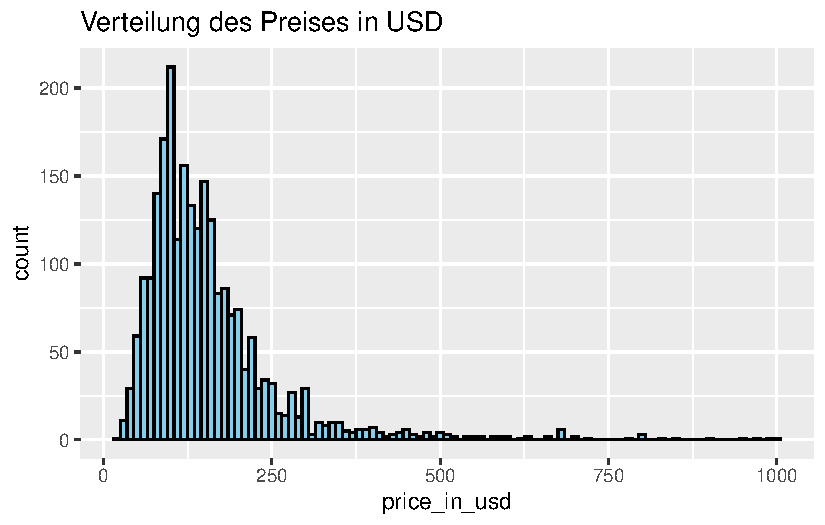
\includegraphics{main_files/figure-pdf/eda-1.pdf}

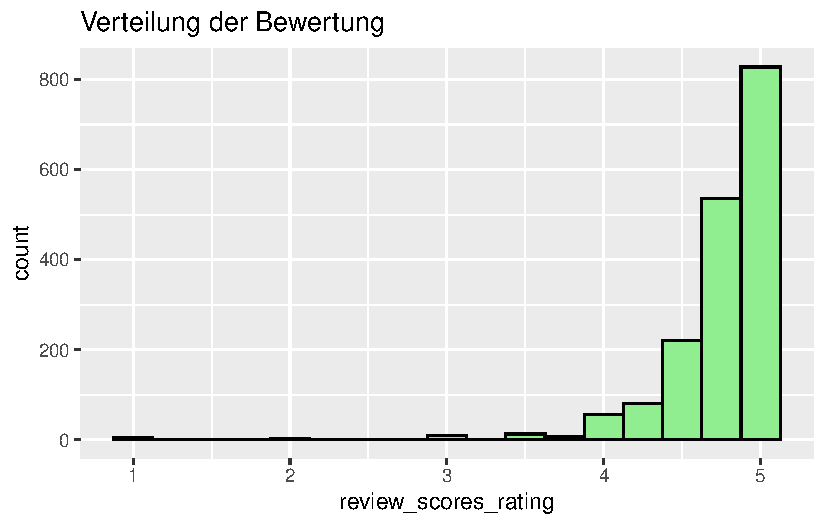
\includegraphics{main_files/figure-pdf/eda-2.pdf}

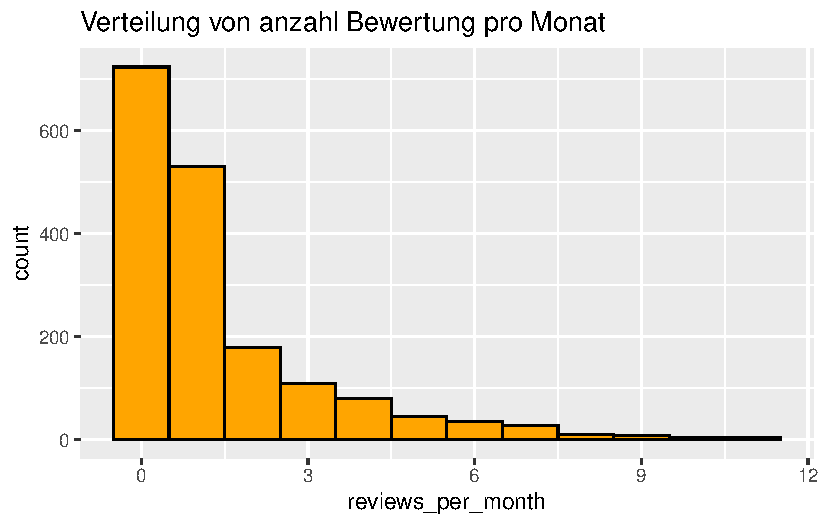
\includegraphics{main_files/figure-pdf/eda-3.pdf}

Da der Preis stark variiert, analysieren wir die Möglichkeit, den Preis
pro Person zu berechnen. Dabei fällt auf, dass der Preis bei ``Entire
home/apt'' für die maximale Anzahl der Gäste
(\textbf{\texttt{accommodates}}) berechnet wird, was sinnvoll ist, da
die gesamte Unterkunft gebucht wird. Bei ``Private room'' und ``Shared
room'' hingegen wird der Preis mehrheitlich pro Person angegeben. Im
Gegensatz dazu ist der Preis bei ``Hotel room'' wieder für die maximale
Gästeanzahl festgelegt.

\hypertarget{datenanalyse-informationen-zur-datenstruktur-organisation-und-zu-den-fuxfcr-die-analyse-verwendeten-methoden}{%
\section{5. Datenanalyse (Informationen zur Datenstruktur, Organisation
und zu den für die Analyse verwendeten
Methoden)}\label{datenanalyse-informationen-zur-datenstruktur-organisation-und-zu-den-fuxfcr-die-analyse-verwendeten-methoden}}

Die bereinigten Datensets der verschiedenen Orten sind alle gleich
aufgebaut. Da wir den Preis der einzelnen Airbnb Apparment anschauen
möchten ist dies unser wichtigster Wert:

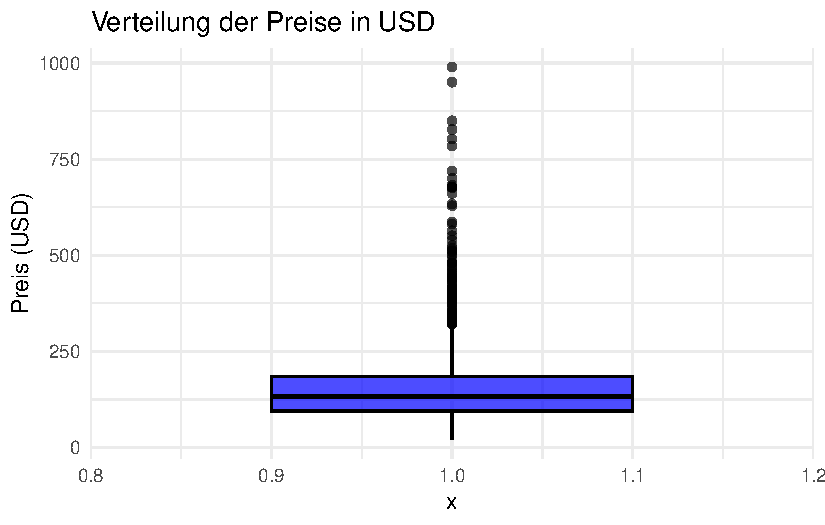
\includegraphics{main_files/figure-pdf/unnamed-chunk-6-1.pdf}

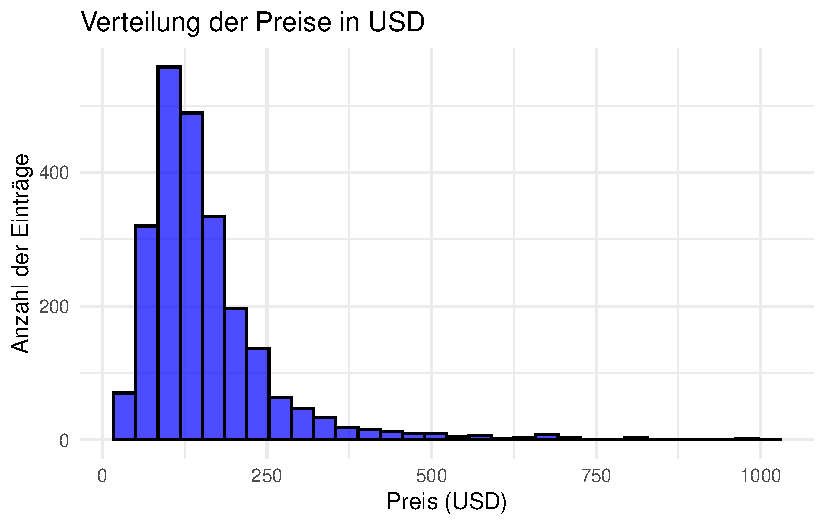
\includegraphics{main_files/figure-pdf/unnamed-chunk-6-2.pdf}

Nun ist stellt sich die Frage welche anderen Eigenschaften die grösste
Auswirkung auf den Preis haben. Dazu gilt es herauszufinden wie die
Korrelationen zwischen dem Preis pro USD und den anderen Attributen
sind:

Die Korrelationen der verschiedenen Variablen mit dem Preis
(\textbf{\texttt{price\_in\_usd}}) im Datensatz können wichtige
Einsichten bieten, welche Faktoren den Preis beeinflussen. Hier ist eine
Analyse der signifikanten positiven und negativen Korrelationen:

\hypertarget{positive-korrelationen}{%
\subsection{\texorpdfstring{\textbf{Positive
Korrelationen:}}{Positive Korrelationen:}}\label{positive-korrelationen}}

\begin{enumerate}
\def\labelenumi{\arabic{enumi}.}
\item
  \textbf{accommodates} (0.449): Es besteht eine moderate positive
  Korrelation zwischen der Anzahl der Gäste, die eine Unterkunft
  aufnehmen kann, und dem Preis. Dies deutet darauf hin, dass grössere
  Unterkünfte, die mehr Gäste beherbergen können, in der Regel teurer
  sind.
\item
  \textbf{beds} (0.329): Eine ähnliche positive Korrelation gibt es
  zwischen der Anzahl der Betten und dem Preis, was darauf hindeutet,
  dass mehr Betten oft höhere Preise bedeuten, was auch mit der Grösse
  der Unterkunft zusammenhängen kann.
\item
  \textbf{availability\_365} (0.157): Längere Verfügbarkeit im Laufe
  eines Jahres korreliert leicht positiv mit höheren Preisen. Dies
  könnte bedeuten, dass Unterkünfte, die seltener verfügbar sind, zu
  höheren Preisen angeboten werden.
\item
  \textbf{last\_scraped} (0.308), \textbf{calendar\_last\_scraped}
  (0.308): Diese Korrelationen deuten darauf hin, dass die Zeitpunkte
  der Datenerfassung mit den Preisänder
\end{enumerate}

\hypertarget{negative-korrelationen}{%
\subsection{\texorpdfstring{\textbf{Negative
Korrelationen:}}{Negative Korrelationen:}}\label{negative-korrelationen}}

\begin{enumerate}
\def\labelenumi{\arabic{enumi}.}
\item
  \textbf{latitude} (-0.097): Es gibt eine leichte negative Korrelation
  zwischen der geographischen Breite und dem Preis. Je weiter nördlich
  die Unterkunft liegt, desto geringer könnte der Preis sein, was auf
  regionale Preisunterschiede in der Stadt oder der Umgebung hinweisen
  könnte.
\item
  \textbf{minimum\_nights} (-0.053), \textbf{first\_review} (-0.053):
  Längere Mindestaufenthalte und frühere erste Bewertungen korrelieren
  leicht negativ mit dem Preis. Dies könnte darauf hinweisen, dass
  preisgünstigere Unterkünfte möglicherweise längere Aufenthalte
  erfordern oder schon länger auf dem Markt sind.
\item
  \textbf{calculated\_host\_listings\_count\_private\_rooms} (-0.103):
  Eine höhere Anzahl von Inseraten, die private Zimmer betreffen,
  korreliert leicht negativ mit dem Preis, was darauf hinweisen könnte,
  dass Gastgeber mit mehreren Einträgen möglicherweise günstigere Preise
  anbieten, um wettbewerbsfähig zu bleiben.
\end{enumerate}

\hypertarget{interpretation}{%
\subsection{\texorpdfstring{\textbf{Interpretation}}{Interpretation}}\label{interpretation}}

\begin{itemize}
\item
  \textbf{Hohe positive Korrelationen} zeigen an, dass mit zunehmender
  Kapazität und Verfügbarkeit der Unterkünfte der Preis steigt. Dies
  reflektiert die Marktlogik, dass grössere und häufiger verfügbare
  Unterkünfte als wertvoller angesehen werden.
\item
  \textbf{Negative Korrelationen} deuten darauf hin, dass bestimmte
  Faktoren wie die geografische Lage (nördlicher) oder die Politik
  längerer Mindestaufenthalte die Preise senken können. Dies könnte für
  Gäste attraktiv sein, die längerfristige Aufenthalte suchen oder
  flexibel in der Wahl der Region sind.
\end{itemize}

Diese Korrelationen sollten jedoch vorsichtig interpretiert werden, da
Korrelation nicht gleich Kausalität ist. Andere verborgene Variablen
könnten ebenfalls eine Rolle spielen, und die Effekte könnten durch
spezifische Marktbedingungen oder andere nicht berücksichtigte Faktoren
beeinflusst werden.

Um diese Korrelationen auch noch grafisch aufzuzeigen mit einer linearen
Regression.

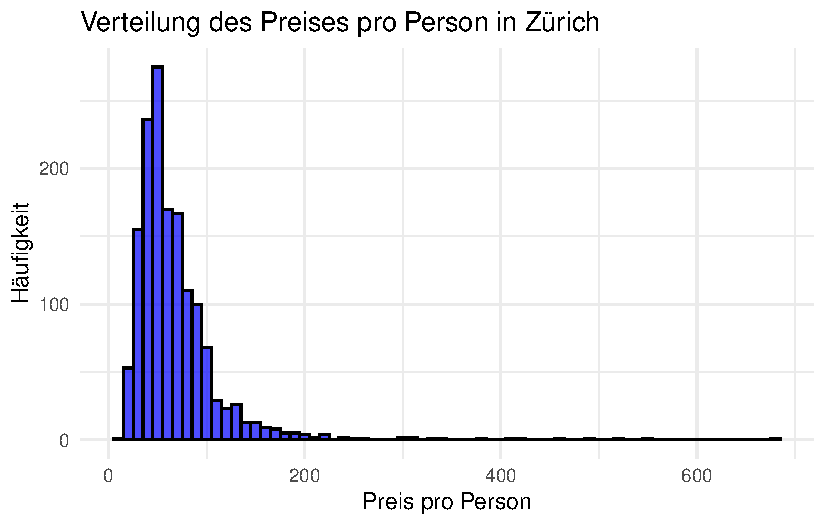
\includegraphics{main_files/figure-pdf/unnamed-chunk-8-1.pdf}

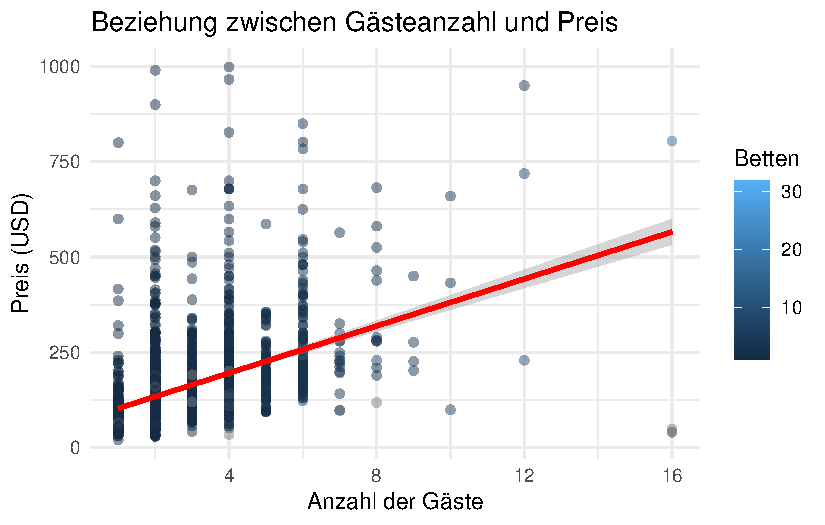
\includegraphics{main_files/figure-pdf/unnamed-chunk-8-2.pdf}

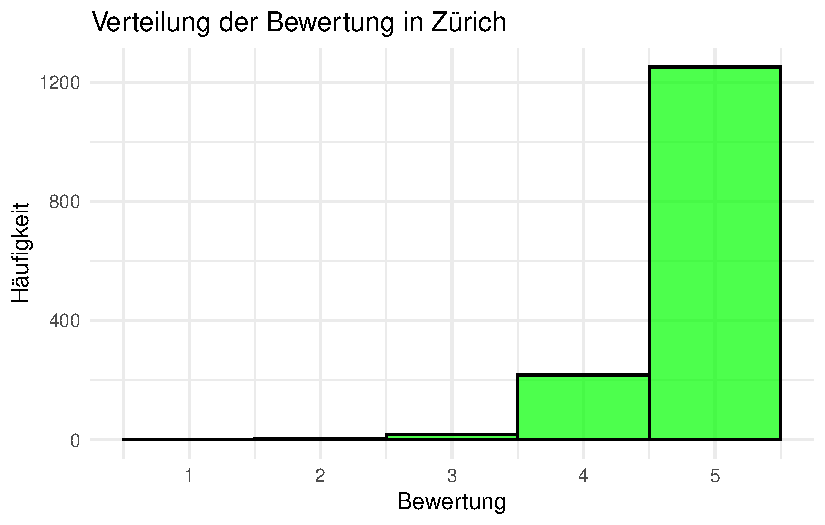
\includegraphics{main_files/figure-pdf/unnamed-chunk-8-3.pdf}

\emph{Die Analyse zeigt auf die irgendwie logische Korrelation zwischen
den Anzahl Gästen respektive Betten und den Preisen eines
AirBNBs\ldots{} Also je grösser das AirBNB desto mehr kostet es\ldots{}}

Gibt es noch andere Korrelationen welche nicht so klar ersichtlich sind?

Vielleicht sind die negativen Beziehungen spannender:

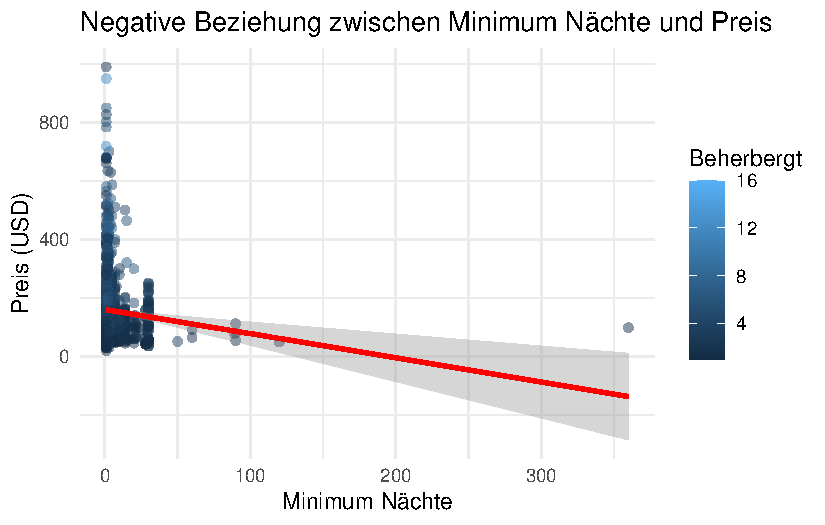
\includegraphics{main_files/figure-pdf/unnamed-chunk-9-1.pdf}

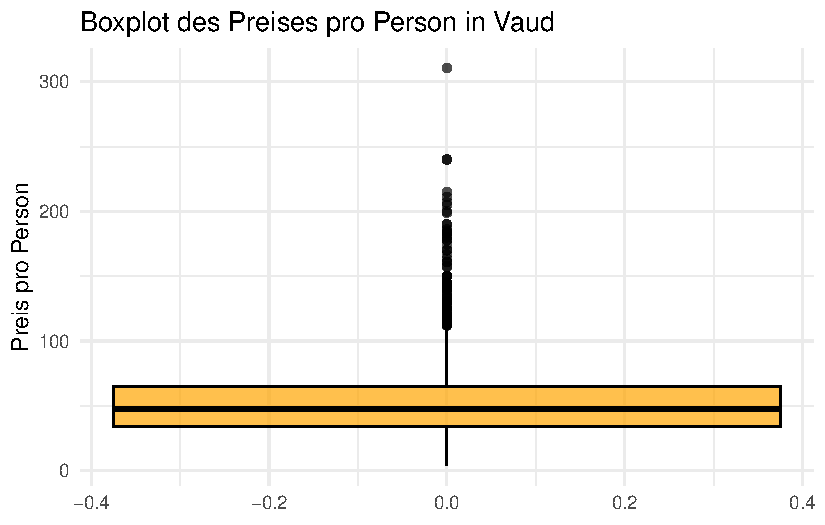
\includegraphics{main_files/figure-pdf/unnamed-chunk-9-2.pdf}

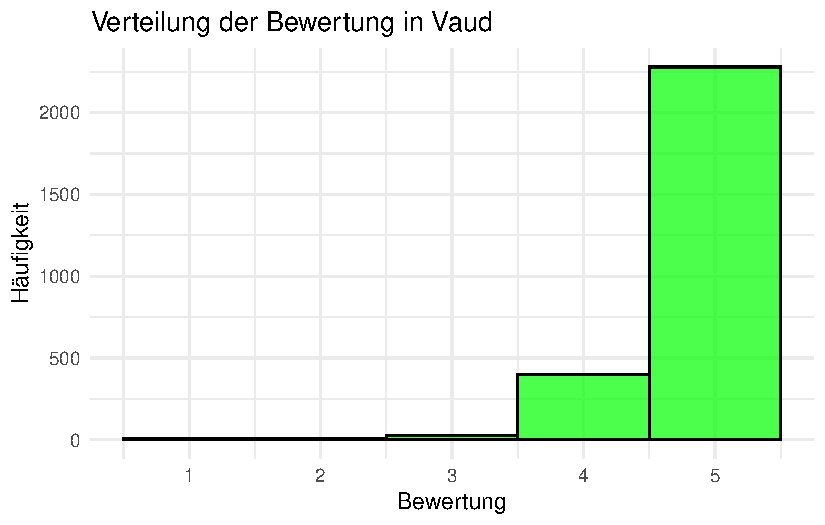
\includegraphics{main_files/figure-pdf/unnamed-chunk-9-3.pdf}

\emph{Sieht schon ein wenig besser aus - vorallem die Latitude. Wobei
auch hier ist es irgendwie klar. Je weiter weg das AirBNB von zentrum
weg ist desto günstiger ist die Wohnung\ldots{}}

\emph{Gibt es sonst noch irgendwelche Möglichkeiten den Preis
vorherauszusagen?}

\begin{verbatim}
RMSE: 41.90135 
\end{verbatim}

\begin{verbatim}
MAE: 27.91819 
\end{verbatim}

\begin{verbatim}
R²: -0.01782196 
\end{verbatim}

\begin{verbatim}
                     IncNodePurity
availability_365          833646.7
review_scores_rating      488147.3
number_of_reviews         718716.6
\end{verbatim}

Die vorliegende Predictive Analyse zielt darauf ab, den Trend des
Preises pro Person einer Unterkunft aufzuzeigen und zu untersuchen, ob
mithilfe der Bewertung und den wichtigsten Eigenschaften einer
Unterkunft eine Prognose über den Preis gemacht werden kann. Dabei
wurden Verfügbarkeit (availability\_365), Bewertung
(review\_scores\_rating) und Anzahl der Bewertungen
(number\_of\_reviews) als Prädiktoren herangezogen.

Die Modellbewertung zeigt folgende Ergebnisse:

\begin{itemize}
\item
  \textbf{RMSE: 41.90135} -- Der durchschnittliche quadratische Fehler
  beträgt 41.90 USD, was auf erhebliche Abweichungen zwischen den
  vorhergesagten und tatsächlichen Preisen hinweist.
\item
  \textbf{MAE: 27.91819} -- Der mittlere absolute Fehler beträgt 27.92
  USD, was ebenfalls auf erhebliche Abweichungen hinweist.
\item
  \textbf{R²: -0.01782196} -- Ein negativer R²-Wert deutet darauf hin,
  dass das Modell die Variation des Preises pro Person nicht gut erklärt
  und kaum besser als zufällige Vorhersagen ist.
\end{itemize}

Die Merkmalswichtigkeit zeigt, dass die Verfügbarkeit über 365 Tage
(IncNodePurity = 833646.7) der wichtigste Prädiktor ist, gefolgt von der
Anzahl der Bewertungen (IncNodePurity = 718716.6) und der Bewertung der
Unterkunft (IncNodePurity = 488147.3). Dies zeigt, dass die
Verfügbarkeit der Unterkunft, die Anzahl der Bewertungen und die
Bewertungen selbst wesentliche Faktoren bei der Preisgestaltung sind.

\hypertarget{ergebnisse-statistische-ergebnisse-zahlen-diagramme}{%
\section{6. Ergebnisse (statistische Ergebnisse, Zahlen,
Diagramme)}\label{ergebnisse-statistische-ergebnisse-zahlen-diagramme}}

\hypertarget{schlussfolgerung-beantwortung-der-frage}{%
\section{7. Schlussfolgerung (Beantwortung der
Frage)}\label{schlussfolgerung-beantwortung-der-frage}}

\hypertarget{referenzen}{%
\section*{8. Referenzen}\label{referenzen}}
\addcontentsline{toc}{section}{8. Referenzen}

\hypertarget{refs}{}
\begin{CSLReferences}{0}{0}
\leavevmode\vadjust pre{\hypertarget{ref-inside-airbnb-2023}{}}%
\CSLLeftMargin{{[}1{]} }%
\CSLRightInline{Inside Airbnb, {``Inside airbnb: Adding data to the
debate,''} 27-Dec-2023. {[}Online{]}. Available:
\url{https://insideairbnb.com/get-the-data/}. {[}Accessed:
30-May-2024{]}}

\leavevmode\vadjust pre{\hypertarget{ref-inside-airbnb-2022}{}}%
\CSLLeftMargin{{[}2{]} }%
\CSLRightInline{Inside Airbnb, {``Inside airbnb data dictionary: Data
dictionary for listings.csV detailed file.''} Aug-2022 {[}Online{]}.
Available:
\url{https://docs.google.com/spreadsheets/d/1iWCNJcSutYqpULSQHlNyGInUvHg2BoUGoNRIGa6Szc4/edit\#gid=1322284596}.
{[}Accessed: 30-May-2024{]}}

\end{CSLReferences}


% Can use something like this to put references on a page
% by themselves when using endfloat and the captionsoff option.
\ifCLASSOPTIONcaptionsoff
  \newpage
\fi

% trigger a \newpage just before the given reference
% number - used to balance the columns on the last page
% adjust value as needed - may need to be readjusted if
% the document is modified later
%\IEEEtriggeratref{8}
% The "triggered" command can be changed if desired:
%\IEEEtriggercmd{\enlargethispage{-5in}}

% Uncomment when use biblatex with style=ieee
%\renewcommand{\bibfont}{\footnotesize} % for IEEE bibfont size

\pagebreak[3]
% that's all folks
\end{document}

